\chapter{Cơ sở lý thuyết và công nghệ}\label{chap:nen}

Chương này giải thích các khái niệm mà thiết kế ở Chương~\ref{chap:thietke} dựa vào: dữ liệu luồng khác dữ liệu tĩnh ở
đâu, Kafka giữ sự kiện thế nào, Spark tổng hợp theo thời gian ra sao khi sự kiện đến lộn xộn, vì sao dữ liệu được lưu
thành ba tầng, và vì sao Cassandra được chọn để phục vụ kết quả.

\section{Bài toán xử lý dữ liệu luồng}\label{sec:luong}
Dữ liệu tĩnh (một file, một bảng) có điểm bắt đầu và kết thúc: chạy truy vấn một lần là có kết quả. Dữ liệu luồng thì
\textbf{không bao giờ kết thúc}: sự kiện đến liên tục, kết quả phải được tính dần và cập nhật mãi. Ngoài ra, mỗi sự kiện
có hai mốc thời gian khác nhau:
\begin{itemize}
  \item \textbf{Event time}: lúc sự việc thật sự xảy ra, ví dụ lúc một người bấm lưu chỉnh sửa trên Wikipedia.
  \item \textbf{Processing time}: thời điểm hệ thống xử lý sự kiện; thời điểm nhận là một mốc khác.
\end{itemize}
Hai mốc này lệch nhau vì mạng chậm, nguồn mất kết nối rồi gửi bù, hay hệ thống tạm dừng. Hình~\ref{fig:eventtime} cho thấy
ba hiện tượng mà mọi hệ thống luồng phải xử lý.

\begin{figure}[H]
\centering
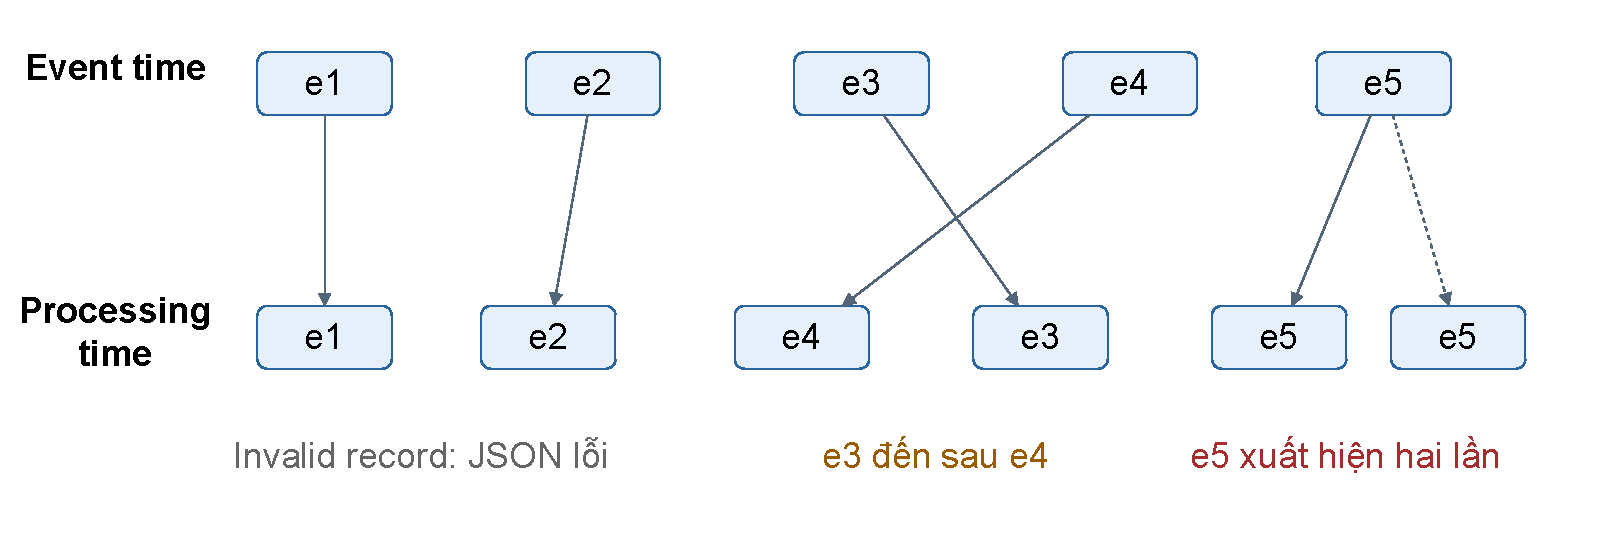
\includegraphics[width=\linewidth]{so-do/theory-01-event-time.pdf}
\caption{Event time và processing time. Mỗi mũi tên nối lúc sự kiện xảy ra với lúc hệ thống xử lý. Sự kiện có thể đến
\textcolor{wpamber}{muộn và lộn thứ tự} (e3), \textcolor{wpred}{đến hai lần} khi nguồn gửi lại (e5), hoặc đến ở dạng
hỏng không đọc được.}\label{fig:eventtime}
\end{figure}

Nếu đếm theo processing time, kết quả phụ thuộc vào việc mạng nhanh hay chậm, và chạy lại cùng dữ liệu sẽ ra số khác.
WikiPulse dùng \textbf{event time} để xếp event vào window theo thời điểm nguồn. Kết quả vẫn phụ thuộc dữ liệu đầu vào, watermark, trạng thái và thứ tự đến; replay không tự bảo đảm cùng kết quả trong mọi điều kiện. Hệ thống cần xử lý late event, bản trùng và bản ghi hỏng. Các mục sau giải thích cách làm từng việc.

\section{Luồng sự kiện thay đổi của Wikipedia}
Wikimedia công bố mọi thay đổi trên các dự án của mình qua dịch vụ EventStreams~\cite{eventstreams}. Client mở một kết nối
HTTP dài và nhận từng sự kiện dạng JSON ngay khi nó xảy ra (giao thức Server-Sent Events). Bảng~\ref{tab:recentchange} liệt
kê các thông tin của một sự kiện mà hệ thống dùng tới.

\begin{table}[H]
\centering\small
\renewcommand{\arraystretch}{1.18}
\caption{Thông tin chính trong một sự kiện thay đổi và cách hệ thống dùng}\label{tab:recentchange}
\begin{tabularx}{\linewidth}{@{}lXX@{}}
\toprule
\textbf{Thông tin} & \textbf{Ý nghĩa} & \textbf{Dùng để} \\ \midrule
Định danh sự kiện & Duy nhất cho mỗi sự kiện & Loại bản trùng \\
Thời điểm & Lúc thay đổi xảy ra (event time) & Xếp vào cửa sổ thời gian \\
Wiki, trang & Ví dụ \enquote{enwiki}, tên bài viết & Nhóm kết quả theo wiki, theo trang \\
Loại thay đổi & Sửa trang, tạo trang mới, ghi nhật ký & Đếm từng loại \\
Kích thước trước, sau & Số byte của trang & Phát hiện xóa nhiều nội dung \\
Người sửa, cờ ẩn danh, cờ bot & Tài khoản hoặc địa chỉ IP và các cờ & Silver băm user với salt; giữ các cờ. Bronze raw giữ payload nguồn \\
\bottomrule
\end{tabularx}
\end{table}

Kết nối dài có thể đứt. Khi nối lại, client có thể nhận lại một phần sự kiện đã nhận, nên phía sau phải chịu được bản
trùng. Ngoài sự kiện thật, Wikimedia còn phát định kỳ \textbf{sự kiện canary} để tự kiểm tra hệ thống của họ; các sự
kiện này phải bị loại khỏi số liệu.
Collector dùng ACK liên tiếp của Kafka để chọn SSE ID khi reconnect trong cùng tiến trình. Cursor chỉ ở bộ nhớ; restart hoặc nguồn không còn giữ vị trí có thể dẫn tới thiếu, trong khi retry có thể tạo bản trùng. Không cam kết exactly-once.

\section{Apache Kafka: bộ đệm sự kiện bền vững}
Kafka~\cite{kreps2011} lưu sự kiện thành một \textbf{nhật ký chỉ ghi thêm} (append-only log). Các khái niệm chính
(Hình~\ref{fig:kafka}):
\begin{itemize}
  \item \textbf{Topic}: một kênh sự kiện, ví dụ kênh chứa các thay đổi thô của Wikipedia.
  \item \textbf{Partition}: topic được chia thành nhiều nhật ký song song để chia tải. Mỗi sự kiện trong một partition có
        số thứ tự tăng dần gọi là \textbf{offset}.
  \item \textbf{Key}: producer gắn key cho mỗi sự kiện; với partitioner và số partition không đổi, cùng key được định tuyến vào cùng partition. Thứ tự được hiểu trong partition, không phải bảo đảm thứ tự toàn hệ thống. WikiPulse dùng key theo wiki và trang.
  \item \textbf{Consumer} tự nhớ mình đã đọc đến offset nào, nên có thể dừng rồi đọc tiếp, hoặc đọc lại từ đầu.
\end{itemize}

\begin{figure}[H]
\centering
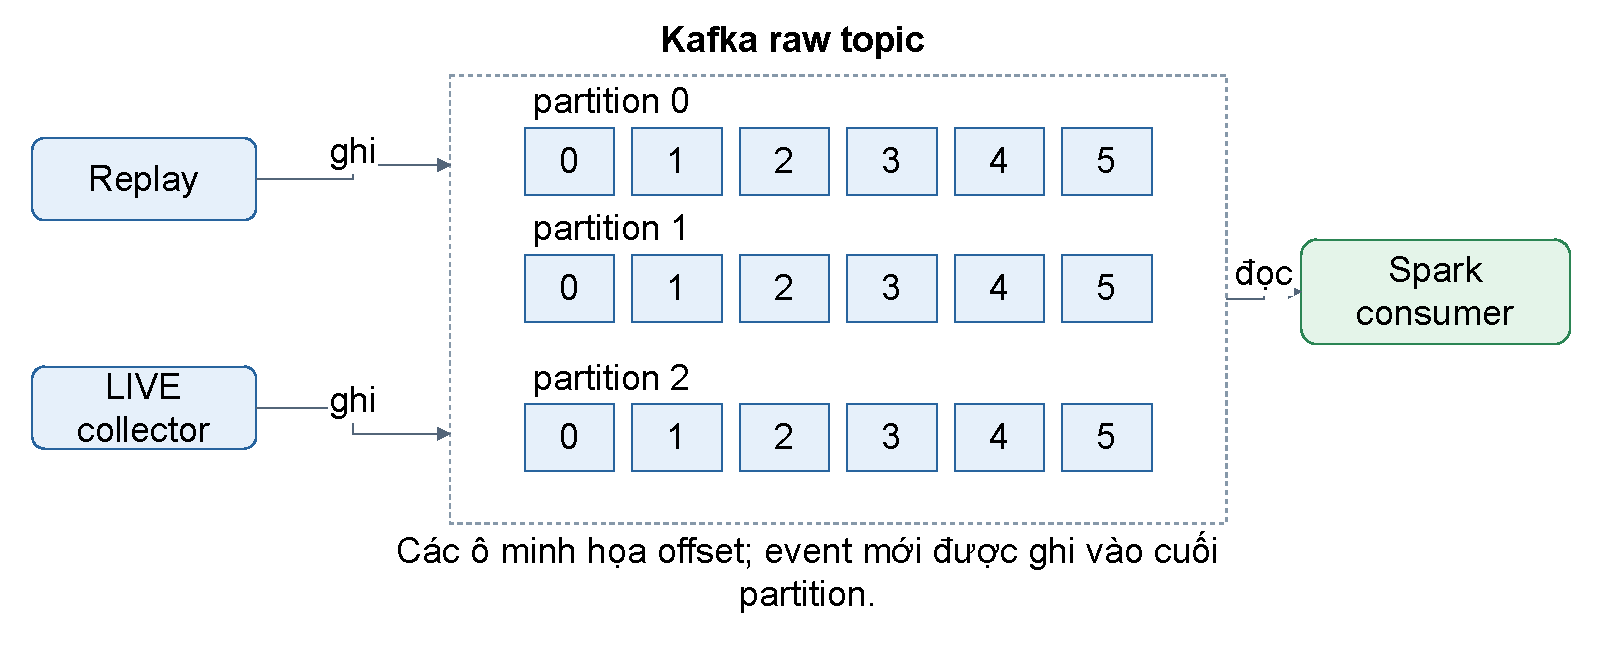
\includegraphics[width=\linewidth]{so-do/theory-02-kafka.pdf}
\caption{Topic Kafka gồm ba partition. Mỗi ô là một sự kiện, số trong ô là offset. Producer ghi vào cuối nhật ký;
consumer (Spark) đọc theo offset và lưu trạng thái theo checkpoint. Collector LIVE đã được triển khai; khả năng tích hợp đầy đủ vẫn cần nghiệm thu.}\label{fig:kafka}
\end{figure}

Trong WikiPulse, Kafka đứng giữa nguồn sự kiện và Spark. Khi Spark dừng, Kafka có thể giữ dữ liệu trong phạm vi retention và trạng thái broker; Spark có thể phục hồi từ checkpoint hợp lệ nếu dữ liệu còn tồn tại. REPLAY ghi fixture vào cùng topic để kiểm thử phần xử lý phía sau; kết quả còn phụ thuộc cấu hình và trạng thái của lần chạy.

\section{Spark Structured Streaming}
\subsection{Mô hình micro-batch}
Spark Structured Streaming~\cite{armbrust2018} cho phép viết truy vấn trên luồng giống như truy vấn trên một bảng bình
thường. Stream được coi là một \textbf{bảng không giới hạn}, mỗi event mới là một dòng thêm vào. Spark dùng trigger
có khoảng mặc định 10 giây trong WikiPulse để lấy dữ liệu mới thành một \textbf{micro-batch}, tính từ state lần trước rồi
ghi kết quả ra đích (Hình~\ref{fig:microbatch}). Nếu batch xử lý lâu, nhịp thực tế có thể chậm hơn cấu hình.

\begin{figure}[H]
\centering
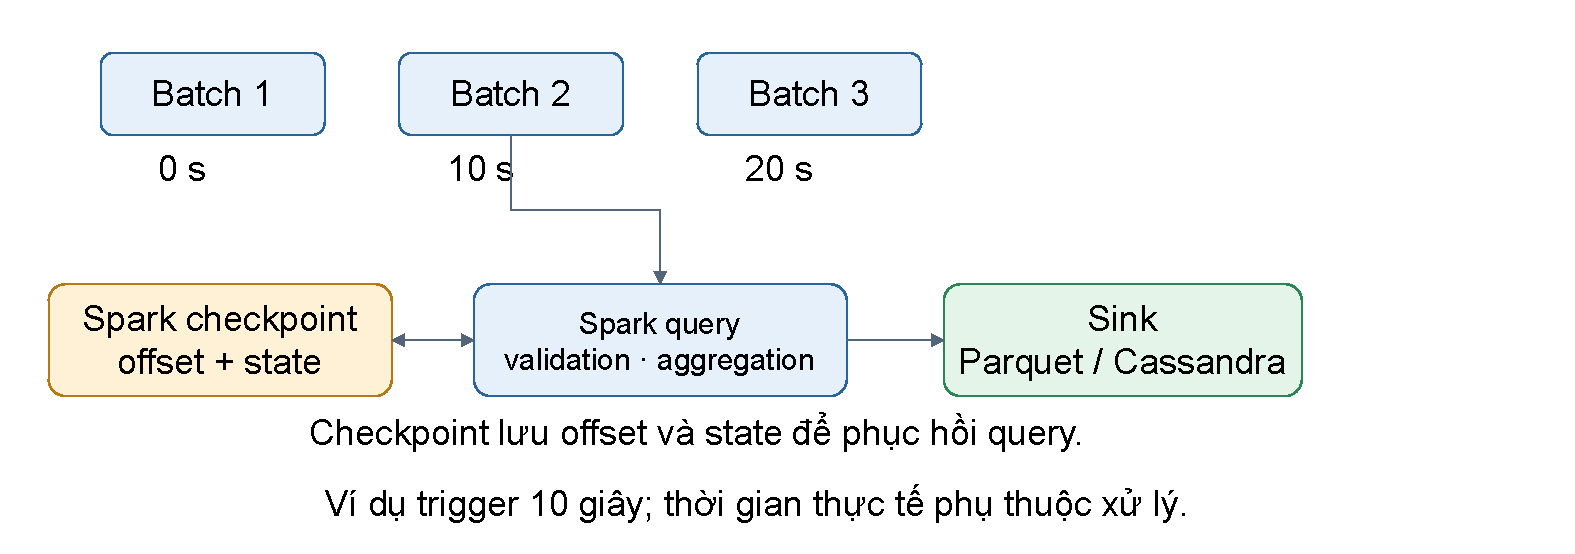
\includegraphics[width=\linewidth]{so-do/theory-03-microbatch.pdf}
\caption{Mô hình micro-batch với trigger mặc định 10 giây; thời điểm thực tế phụ thuộc thời gian xử lý. Query kết hợp batch với state trong checkpoint.}\label{fig:microbatch}
\end{figure}

\textbf{Checkpoint} lưu hai thứ: đã đọc Kafka tới offset nào, và trạng thái đang tính dở (ví dụ số đếm của các cửa sổ chưa
chốt). Spark có thể phục hồi từ checkpoint hợp lệ nếu nguồn còn dữ liệu và state/schema tương thích. Checkpoint gắn chặt với cấu trúc
truy vấn: đổi cách tính có trạng thái thì phải dùng checkpoint mới.

\subsection{Window và watermark}
Để đếm \enquote{mỗi phút có bao nhiêu chỉnh sửa}, sự kiện được xếp vào các \textbf{cửa sổ} 1 phút theo event time. Câu hỏi
khó là: \emph{khi nào thì một cửa sổ được coi là đủ?} Sự kiện của phút 00:00 có thể vẫn đang trên đường tới. Spark trả
lời bằng \textbf{watermark}~\cite{akidau2015}:
\[
  \text{watermark} = \text{event time lớn nhất đã thấy} - \text{độ trễ cho phép (10 phút)}.
\]
Khi watermark tiến qua cuối window, query có thể xuất kết quả finalized theo output mode. Sự kiện đến quá muộn có thể bị loại khỏi phép tính có state, trong khi Bronze raw vẫn giữ bản ghi Kafka. Watermark dựa trên event time quan sát được và tiến độ query, không phải timer theo đồng hồ; khi stream im lặng không thể giả định Gold lập tức được chốt.
Hình~\ref{fig:watermark} minh họa bằng chính dữ liệu mẫu của dự án.

\begin{figure}[H]
\centering
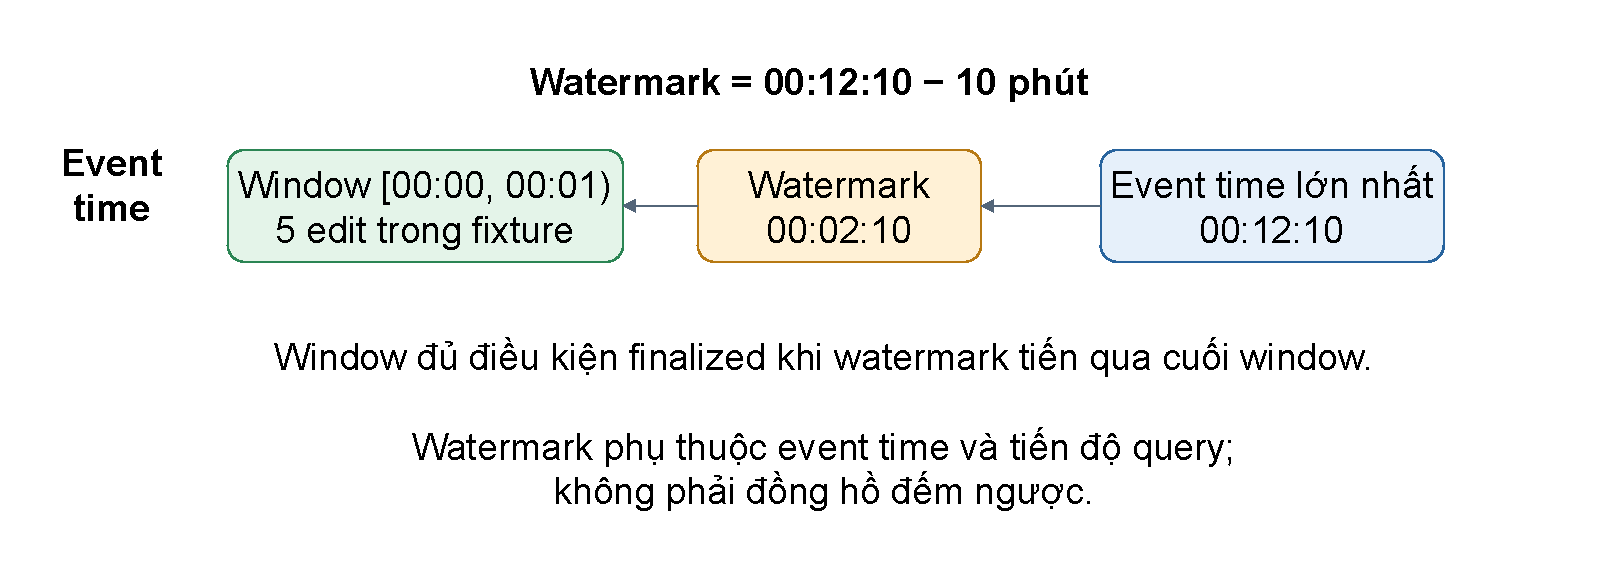
\includegraphics[width=\linewidth]{so-do/theory-04-watermark.pdf}
\caption{Watermark trên dữ liệu mẫu. Sự kiện lúc 00:12:10 đẩy watermark tới 00:02:10, nên cửa sổ 00:00 (5 chỉnh sửa
enwiki) được chốt. Các window có cuối sau watermark này chưa đủ điều kiện finalized chỉ dựa trên mốc đó.}\label{fig:watermark}
\end{figure}

Độ trễ cho phép là một sự đánh đổi: dài thì đếm được nhiều sự kiện muộn hơn nhưng phải giữ nhiều trạng thái và chờ lâu
mới có số chốt; ngắn thì ngược lại. Dự án chọn 10 phút.

\subsection{Số tạm tính và số đã chốt}
Người xem dashboard muốn thấy số ngay, không muốn chờ 10 phút. Spark có hai \textbf{chế độ xuất} kết quả, và WikiPulse
dùng cả hai cho cùng một phép đếm (Bảng~\ref{tab:chedo}).

\begin{table}[H]
\centering\small
\caption{Hai chế độ xuất kết quả}\label{tab:chedo}
\begin{tabularx}{\linewidth}{@{}lXXX@{}}
\toprule
\textbf{Chế độ} & \textbf{Khi nào ghi} & \textbf{Tính chất} & \textbf{Đích trong WikiPulse} \\ \midrule
Update & Mỗi batch, mọi cửa sổ vừa thay đổi & Nhanh; số còn có thể tăng (tạm tính) & Activity: Cassandra; trends: Parquet hoặc Cassandra theo cấu hình \\
Append & Khi window đủ điều kiện theo watermark & Kết quả finalized; thời điểm xuất phụ thuộc tiến độ event time & Tầng Gold, cho phân tích \\
\bottomrule
\end{tabularx}
\end{table}

Spark có một giới hạn quan trọng: một truy vấn ở chế độ Update không được chứa hai bước cần nhớ trạng thái liên tiếp, ví
dụ \enquote{loại trùng rồi đếm}~\cite{sparkguide}. Vì vậy WikiPulse tách thành nhiều truy vấn: một truy vấn loại trùng và
ghi ra đĩa, các truy vấn khác đọc lại kết quả đó để đếm (Mục~\ref{sec:spark}).

\subsection{Loại bản trùng}
Mỗi sự kiện có một định danh duy nhất. Spark nhớ các định danh đã thấy và bỏ sự kiện nào trùng. Không thể nhớ mãi, nên
Spark dùng event ID và state có watermark để deduplication trong phạm vi cấu hình. Bản trùng đến muộn có thể bị bỏ vì quá muộn hoặc không còn được nhận diện là trùng; không khẳng định chính xác kết quả mọi trường hợp hay exactly-once.

\section{Kiến trúc dữ liệu ba tầng}
Thay vì chỉ lưu kết quả cuối, dữ liệu được lưu theo ba tầng~\cite{medallion}, mỗi tầng sạch hơn tầng trước
(Hình~\ref{fig:medallion}). Lưu tầng thô giúp kiểm tra lại khi nghi có lỗi và tính lại khi đổi công thức mà không cần nguồn
gửi lại dữ liệu.

\begin{figure}[H]
\centering
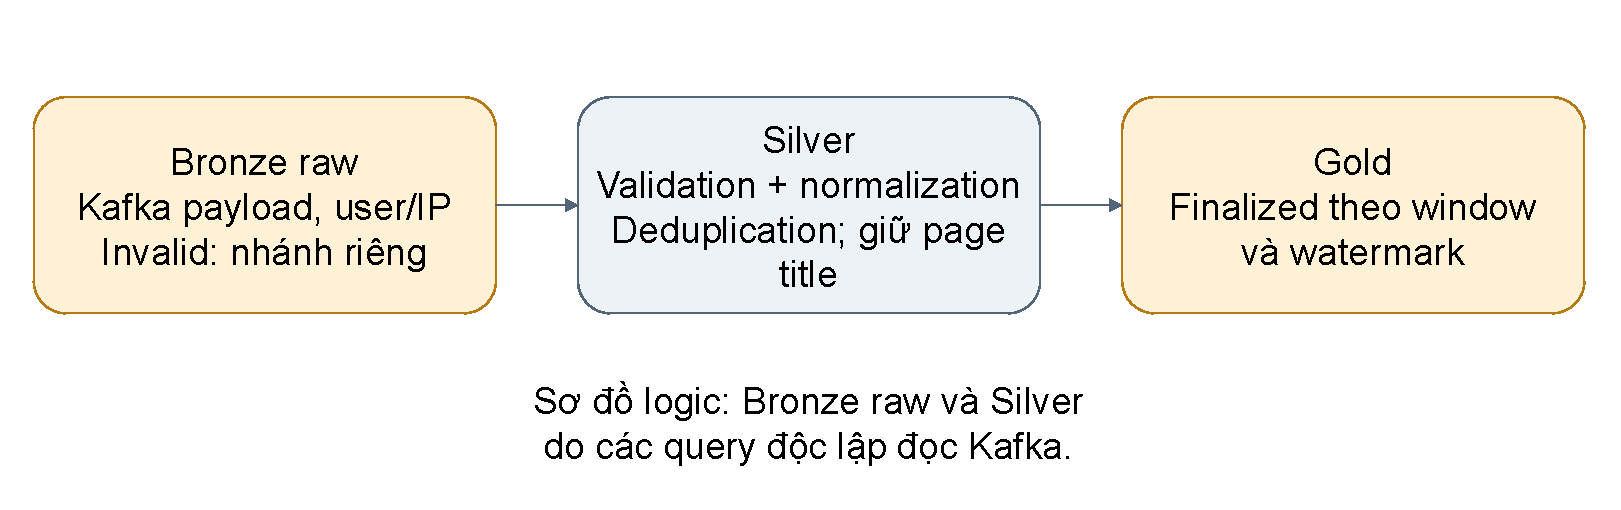
\includegraphics[width=\linewidth]{so-do/theory-05-medallion.pdf}
\caption{Ba tầng dữ liệu. Đi từ trái sang phải, dữ liệu sạch dần và ít thông tin nhạy cảm hơn.}\label{fig:medallion}
\end{figure}

Ba tầng được lưu dạng \textbf{Parquet}, định dạng theo cột, nén tốt, đọc nhanh khi chỉ cần vài cột. File được chia thư
mục theo ngày và giờ, nên truy vấn một khoảng thời gian chỉ phải đọc đúng các thư mục đó.

\section{Apache Cassandra: phục vụ kết quả}
Dashboard cần đọc số liệu nhanh, liên tục. Parquet hợp cho phân tích theo lô nhưng không hợp để trả lời hàng nghìn câu
hỏi nhỏ mỗi phút. Kết quả tạm tính vì vậy được ghi vào Cassandra~\cite{lakshman2010}.

Khác CSDL quan hệ, trong Cassandra \textbf{bảng được thiết kế theo câu truy vấn}, không theo thực thể~\cite{cassandracql}.
Khóa chính có hai phần (Hình~\ref{fig:cassandra}):
\begin{itemize}
  \item \textbf{Partition key} quyết định dữ liệu nằm cùng nhau ở đâu. WikiPulse dùng wiki: mọi cửa sổ của enwiki nằm
        chung một partition.
  \item \textbf{Clustering key} quyết định thứ tự trong partition. WikiPulse dùng thời điểm bắt đầu cửa sổ, sắp giảm dần,
        nên các phút mới nhất luôn nằm đầu.
\end{itemize}

\begin{figure}[H]
\centering
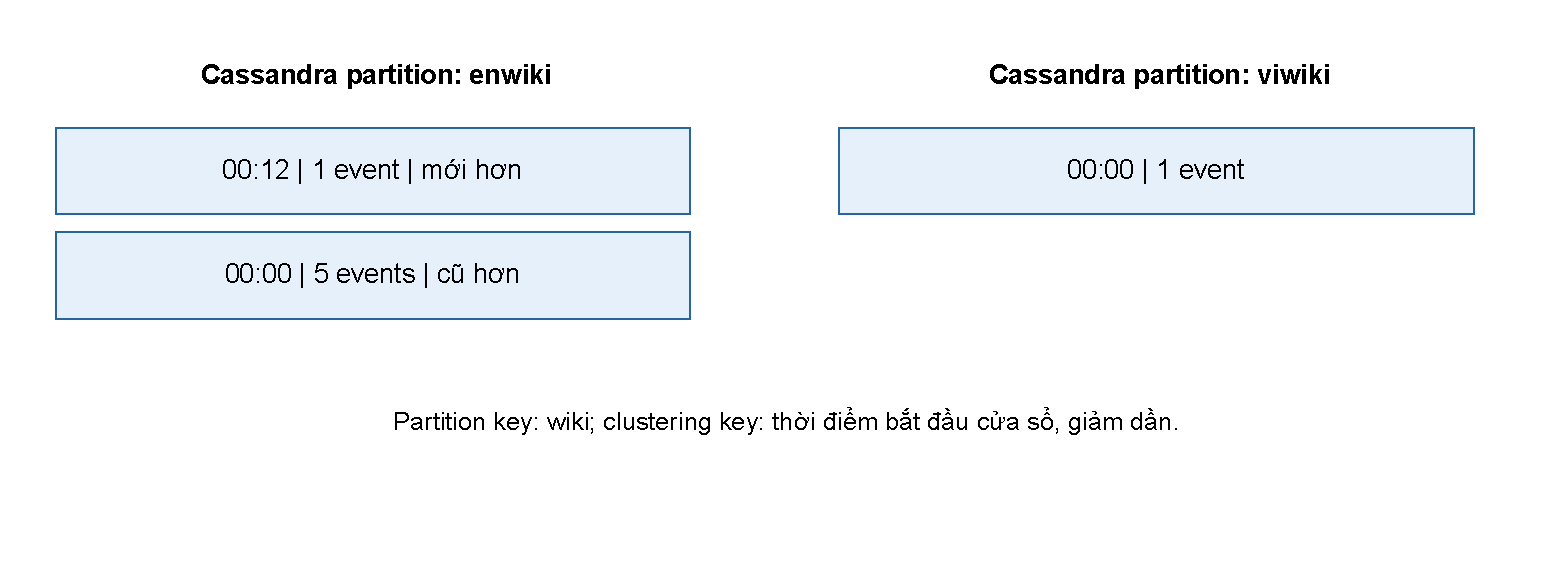
\includegraphics[width=\linewidth]{so-do/theory-06-cassandra.pdf}
\caption{Dữ liệu hoạt động trong Cassandra. Mỗi wiki là một partition; trong partition, các cửa sổ xếp mới trước.}\label{fig:cassandra}
\end{figure}

Hai tính chất của Cassandra quyết định cách ghi:
\begin{itemize}
  \item Ghi một dòng có khóa đã tồn tại thì \textbf{ghi đè} (upsert), không sinh dòng mới. WikiPulse ghi \emph{tổng số}
        của cửa sổ chứ không ghi \enquote{cộng thêm 1}, nên khi Spark ghi lại một batch sau sự cố, kết quả vẫn đúng, không
        bị đếm đôi.
  \item Truy vấn không chỉ rõ partition buộc Cassandra quét mọi node. Dự án cấm kiểu truy vấn này (\enquote{allow
        filtering}); mỗi câu hỏi của API phải có bảng thiết kế riêng cho nó.
\end{itemize}

\section{FastAPI và Streamlit}
\textbf{FastAPI} là framework Python để viết API web; kiểu dữ liệu khai báo một lần được dùng để kiểm tra đầu vào, định
dạng đầu ra và sinh tài liệu API tự động (OpenAPI). \textbf{Streamlit} dựng giao diện dashboard bằng Python thuần, hợp với
nhóm không có người chuyên frontend.

\section{Công nghệ sử dụng}
\begin{table}[H]
\centering\small
\caption{Công nghệ sử dụng và vai trò}\label{tab:congnghe}
\begin{tabularx}{\linewidth}{@{}llX@{}}
\toprule
\textbf{Thành phần} & \textbf{Lựa chọn} & \textbf{Vai trò} \\ \midrule
Hàng đợi & Apache Kafka 3.9 & Giữ sự kiện, tách nguồn khỏi xử lý, cho phép đọc lại \\
Xử lý luồng & Spark 3.5 (PySpark) & Kiểm tra, chuẩn hóa, loại trùng, đếm theo cửa sổ \\
Lưu trữ phân tích & Parquet (local hoặc HDFS) & Ba tầng Bronze, Silver, Gold \\
Lưu trữ phục vụ & Apache Cassandra 4.1 & Số tạm tính cho API \\
API & FastAPI & Cung cấp số liệu cho dashboard \\
Giao diện & Streamlit & Dashboard bốn trang \\
Chạy & Docker Compose & Dựng toàn bộ hệ thống bằng một lệnh, chạy trên ARM64 và x86\_64 \\
Ngôn ngữ, kiểm thử & Python 3.11, pytest & Toàn bộ mã nguồn và kiểm thử \\
\bottomrule
\end{tabularx}
\end{table}
Profile full bổ sung HDFS cho data và Spark checkpoint; cấu hình mặc định vẫn dùng local storage.

% ============================================================================
% CHƯƠNG 3: LIÊN QUAN
% ============================================================================
